\documentclass[../CSC_5RO07_TA.tex]{subfiles}

\begin{document}
\section{Q1: Network on Chip 3x3}

Le Network on Chip (NoC) est un concept clé dans les systèmes multiprocesseurs sur puce (MPSoC), abordé dans le cadre de la matière "Multiprocesseurs sur puce". Il s'agit d'une solution d'interconnexion utilisant un réseau de routeurs et de liens pour assurer une communication efficace entre les différents cœurs de traitement et autres modules intégrés sur une même puce. Pendant les travaux pratiques avec la ZedBoard, cette technologie est étudiée pour comprendre comment les topologies de NoC optimisent les performances, l'évolutivité et l'efficacité énergétique dans des systèmes embarqués complexes.

\begin{figure}[H]
    \centering
    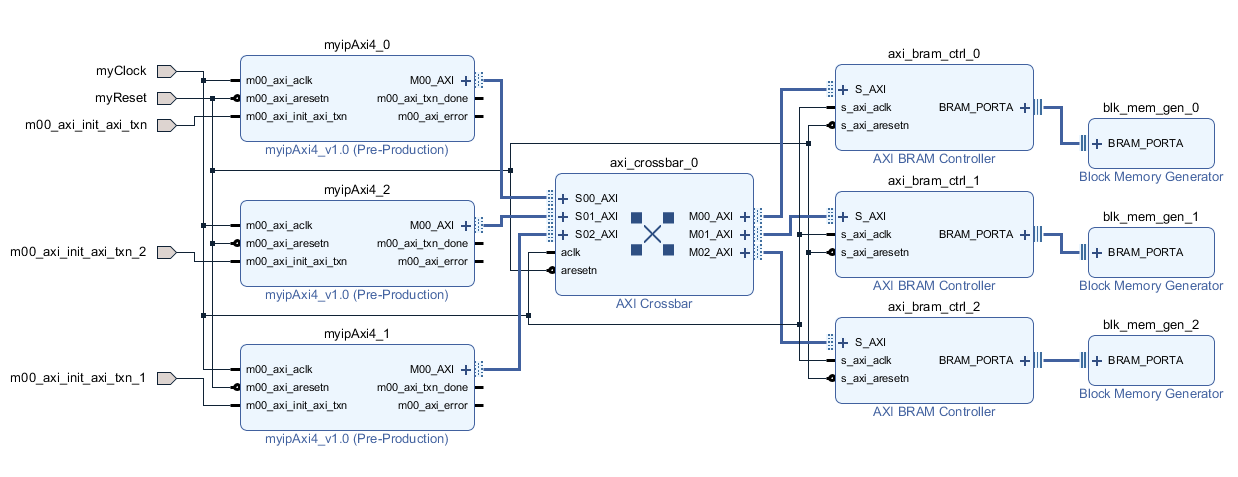
\includegraphics[width=0.75\textwidth]{./images/Q1-1.png}
    \caption{Implémentation Full Crossbar.}
\end{figure}

Le projet est appelé NoC 3x3 en raison de son architecture suivant une topologie en grille 3x3, où trois éléments principaux (comme les modules "myip\_v1.0") sont interconnectés à trois contrôleurs de mémoire BRAM via un AXI Crossbar. Cette configuration reflète l’organisation typique d’un Network on Chip, où chaque nœud du réseau peut communiquer efficacement avec les autres, garantissant une haute scalabilité et performance. Cette topologie a été implémentée et validée dans le projet à l’aide de la ZedBoard.

\subsection{Mise en œuvre et validation du NOC 3x3 avec générateurs de trafic}

Pour tester et valider le NoC 3x3, l’exemple disponible sur le drive du cours a été téléchargé à partir du dossier ``crossBar", qui contient trois sous-dossiers supplémentaires. Pour cette étape, ainsi que pour le calcul de la latence et de la bande passante, le modèle ``crossbarSimple" a été utilisé, ce dernier n'étant pas encore relié à la carte. Le fichier ouvert pour les simulations se trouve à l'emplacement suivant : ``/crossBar/crossbarSimple/axiCrossBar/axiCrossBar.xpr". Pendant le processus, il a été nécessaire de permettre à l'application de mettre à jour certains IPs pour qu'ils soient compatibles avec la version actuelle. Enfin, la simulation (behavioral simulation) a été exécutée pour observer les résultats de trafic, lesquels peuvent également être visualisés à partir de l’onglet ``Flow".

\begin{figure}[H]
    \centering
    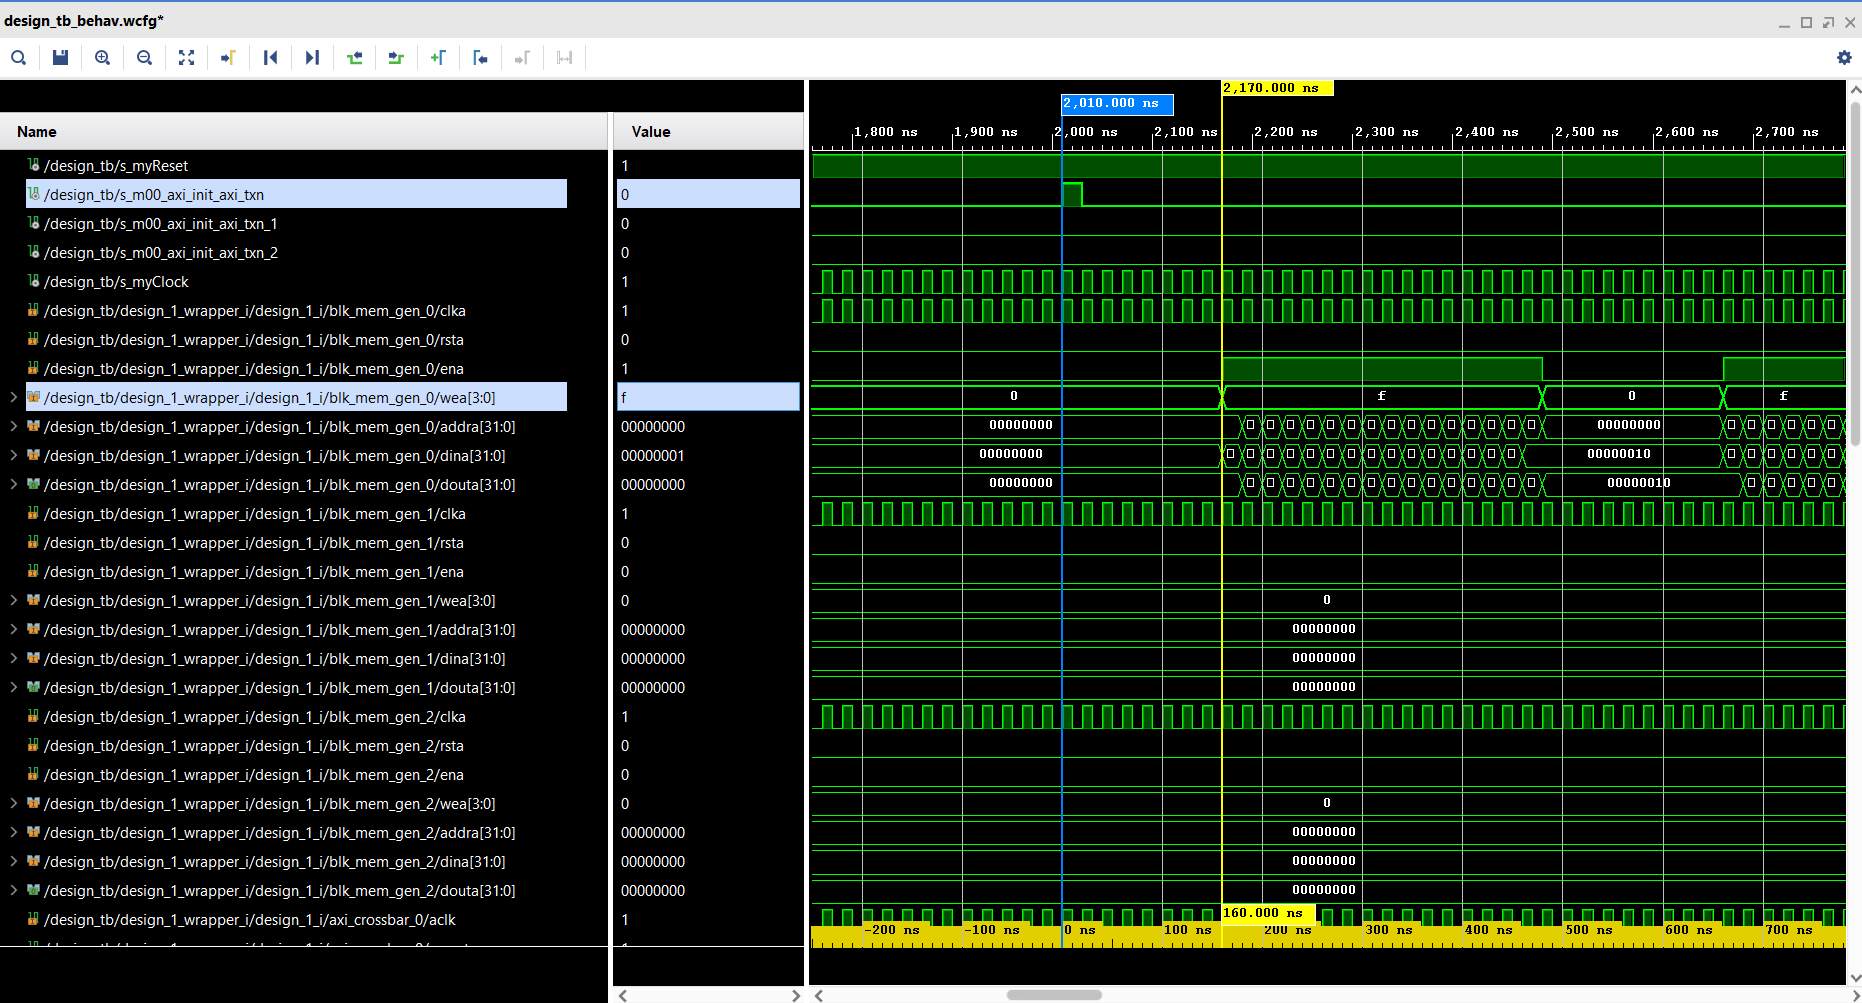
\includegraphics[width=0.8\textwidth]{./images/behaviorSim.png}
    \caption{Écran de la ``Behavior Simulation''.}
    \label{BS20ns}
\end{figure}


\subsection{Analyse de la latence et de la bande passant}

L’analyse de la latence et de la bande passante du NoC 3x3 prend en compte le concept de "slack", qui correspond à la différence de temps entre le début du prochain cycle d’horloge et le début de la réponse au signal. Si le slack est positif, la réponse intervient avant le deuxième cycle d’horloge ; s’il est négatif, elle intervient après. La latence, quant à elle, est définie comme l’intervalle entre l’entrée d’un signal dans le générateur de trafic (TX) et son écriture dans la mémoire BRAM, ce qui indique que les données ont été correctement enregistrées. Cette latence est influencée par le temps de programmation du système. Pour l’analyse, un burst de 256 mots de 32 bits a été considéré, avec une fréquence d’horloge de 100 MHz (10 ns). Les résultats de la simulation, observés sur l’écran de la Behavioral Simulation, montrent que la latence mesurée est d’environ 80 ns.

\begin{figure}[H]
    \centering
    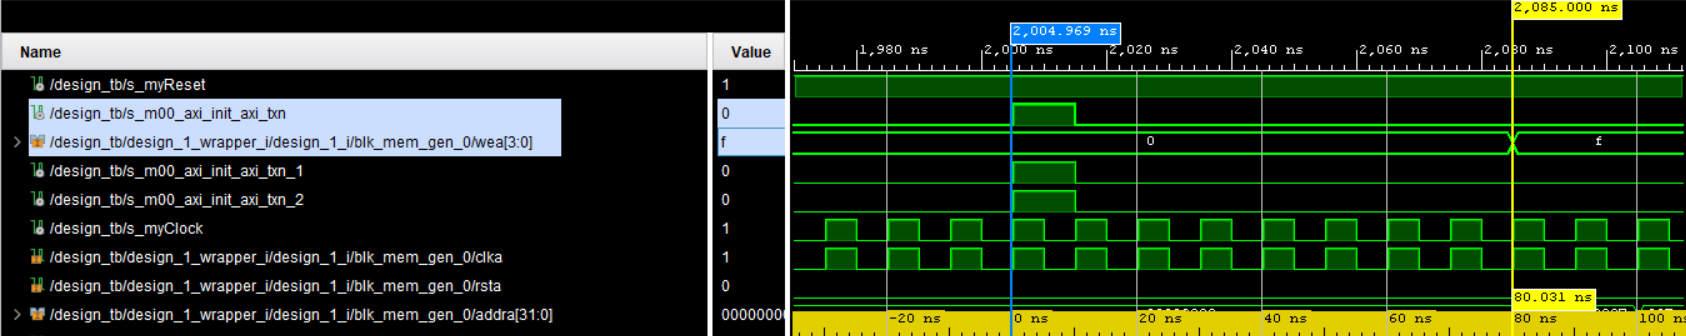
\includegraphics[width=0.8\textwidth]{./images/latencia10ns.png}
    \caption{Mésurement de la latence sur l'écran ``Behavior Simulation''.}
    \label{BS10ns}
\end{figure}

La bande passante est la capacité maximale de transmission de données dans un système pendant un intervalle de temps donné, généralement mesurée en bits par seconde (bps). Dans le contexte du NoC, elle indique le volume de données pouvant être transféré entre les composants. Elle représente la capacité du canal de communication et est directement liée à l’efficacité du système.

\[
\text{Bande passante} = \frac{\text{Volume total de données (bits)}}{\text{Temps total de transfert (secondes)}}
\]


\begin{itemize}
    \item \textbf{Volume total de données} : Chaque transfert de données comprend 256 mots, et chaque mot contient 32 bits. Ainsi, le volume total de données est donné par :
    \[
    \text{Volume total de données} = 256 \times 32 = 8192 \, \text{bits}.
    \]

    \item \textbf{Temps total de transfert} : Chaque transfert de mot prend 10 \textit{ns}. Le temps total pour transférer 256 mots est donc :
    \[
    \text{Temps total de transfert} = 256 \times 10 \, \text{ns} = 2560 \, \text{ns} = 2.56 \times 10^{-6} \, \text{s}.
    \]
\end{itemize}

En appliquant ces valeurs à la formule, nous obtenons :
\[
\text{Bande passante} = \frac{8192}{2,56 \times 10^{-6}} = 3.2 \, \text{Gbps}.
\]

Ainsi, la bande passante mesurée pour ce système est de 3 x \textbf{3.2 Gbps} = \textbf{9.6 Gbps}.


 
\subsection{NOC sur Zynq}

La figure suivante présente l'implementation du circuit NOC sur Zynq. 

\begin{figure}[H]
    \centering
    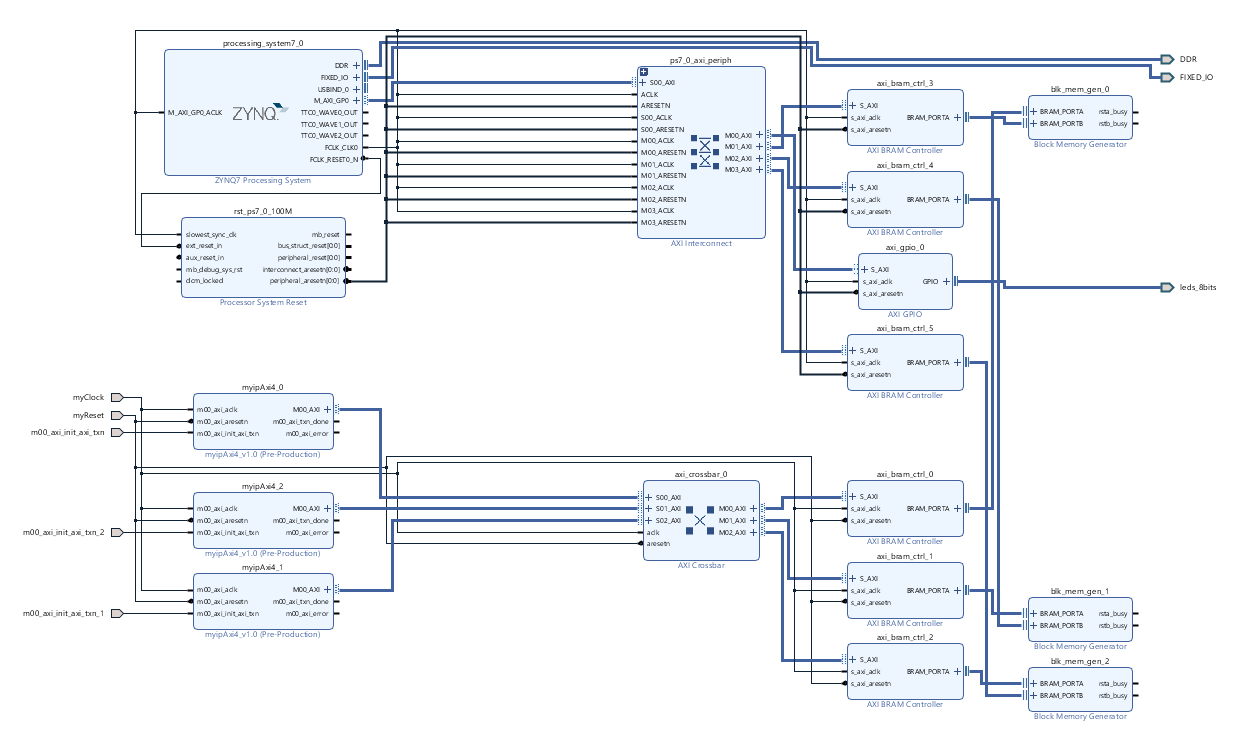
\includegraphics[width=1\textwidth]{./images/NOCZYNQ.png}
    \caption{NOC sur ZYNQ}
\end{figure}

Lié aux blocs de mémoire BRAM, nous trouvons les blocs de gestion de mémoire, ceux qu'iront s'en charger de synchroniser les opérations d'accès mémoire, sachant que les deux parties du circuit peuvent opérer à différents fréquences d'horloge. En plus, l'AXI Interconnect est responsable pour le traitement des données sortantes du Processeur Zynq et les mémoires et GPIO.

Les configurations de Crossbar Full-Access et Shared Access ont été testées pour vérifier leur utilisation de ressources. La stratégie Synthesis Performance Net Delay Low a eté choisi pour vérifier si le chemin de connexions dans le circuit pourrait changer pour un nouveau critère de synthèse: 

\begin{figure}[H]
    \centering
    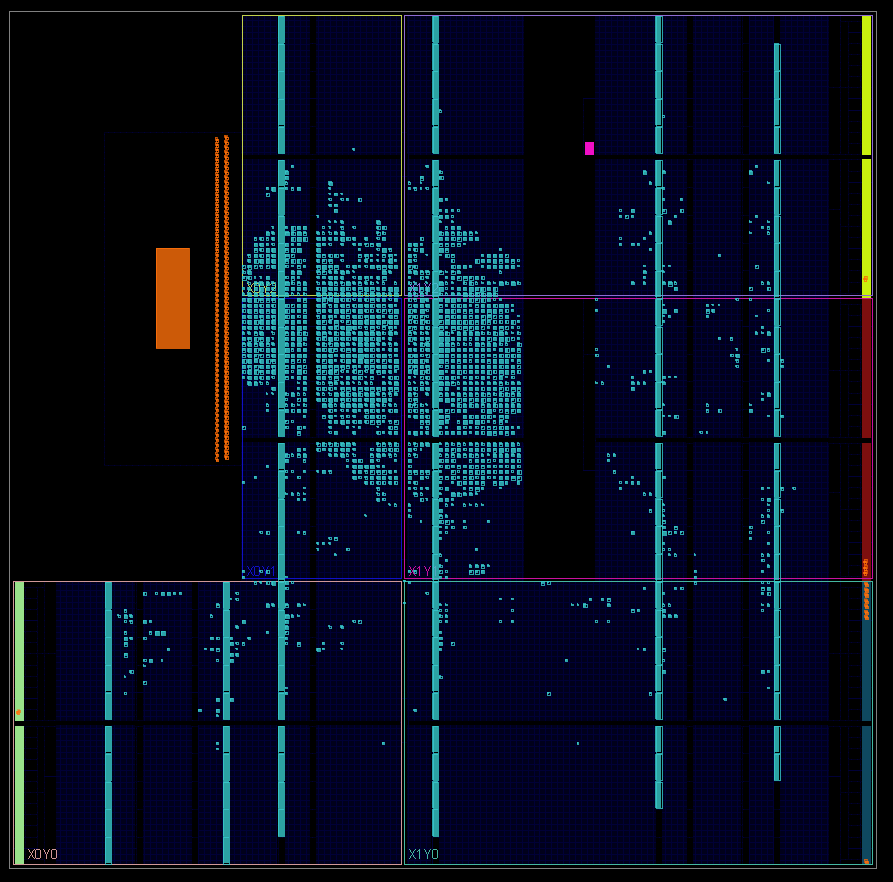
\includegraphics[width=0.6\textwidth]{./images/perfNetDelLow_full_imp.png}
    \caption{Implémentation Full-Access Crossbar.}
\end{figure}

\begin{figure}[H]
    \centering
    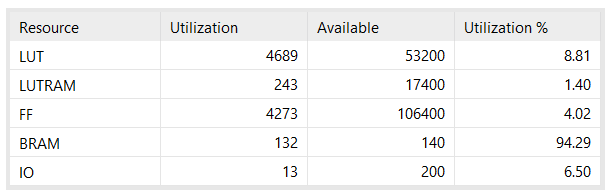
\includegraphics[width=0.6\textwidth]{./images/perfNetDelLow_full_uti.png}
    \caption{Utilisation des ressources pour la configuration Full-Access crossbar.}
\end{figure}

\begin{figure}[H]
    \centering
    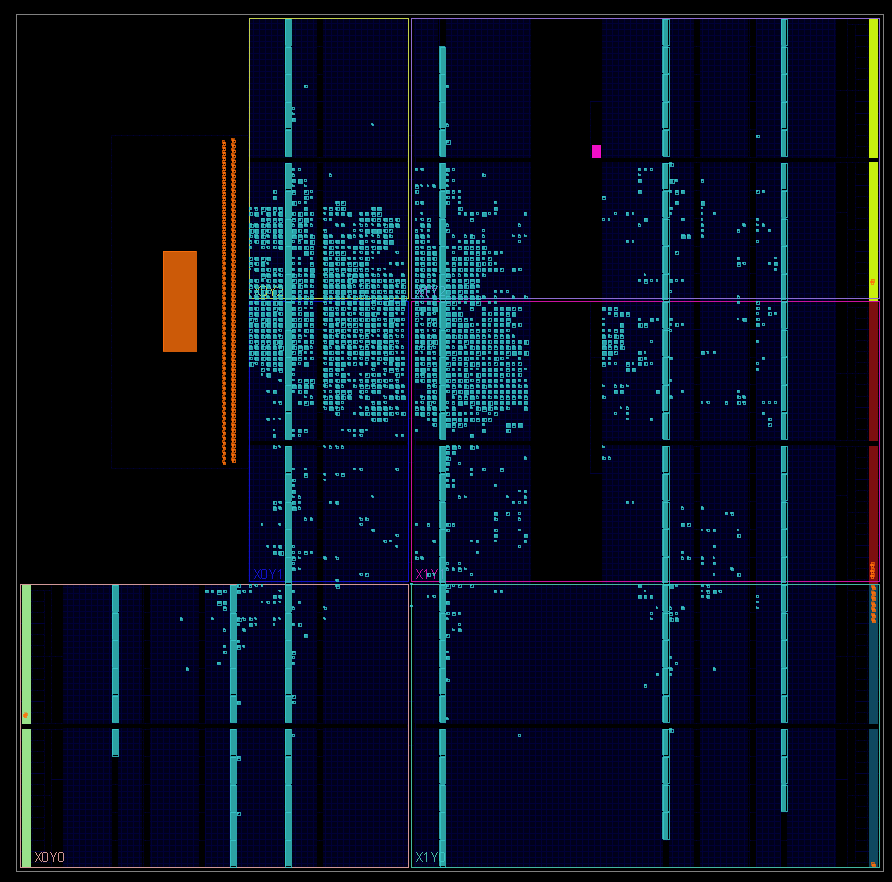
\includegraphics[width=0.6\textwidth]{./images/perfNetDelLow_shared_imp.png}
    \caption{Implémentation Shared-Acess Crossbar.}
\end{figure}

\begin{figure}[H]
    \centering
    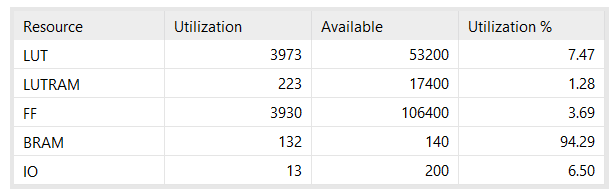
\includegraphics[width=0.6\textwidth]{./images/perfNetDelLow_shared_uti.png}
    \caption{Utilisation des ressources pour la configuration Shared-Acess Crossbar.}
\end{figure}

Vu que les ressources BRAM et IO restent égales à cause de la fixation de l'architecture en termes de conexions et mémoire, la légère différence entre ressources (surtout les LUT) ne doit pas justifier le changement de configuration Crossbar, sachant que la Shared-Access est bien moins performant.

Finalement, les stratégies de synthèse ont faire varier plus considérablement les ressources utilisés pour la configuration Full-Access Crossbar, Même si la proportion générale entre ressources a resté similaire. L'optimisation de Area peut bien réduire, en termes proportionnels, l'utilisation des LUT, LUTRAM et FF; néanmoins, cette option a comme effet une réduction de performance:

\begin{figure}[H]
    \centering
    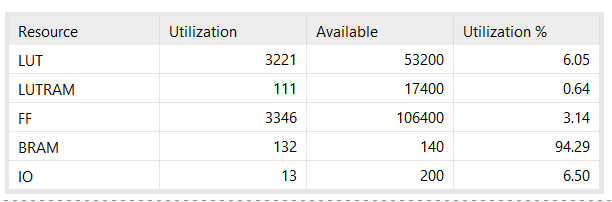
\includegraphics[width=0.6\textwidth]{./images/area optimize high.png}
    \caption{Synthesis Area Optimize High.}
\end{figure}

\begin{figure}[H]
    \centering
    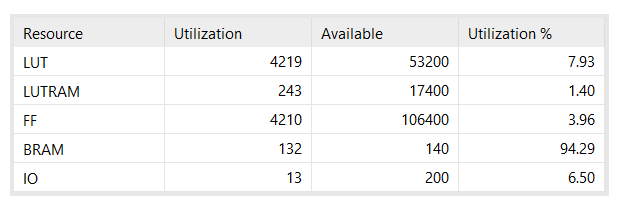
\includegraphics[width=0.6\textwidth]{./images/performance optimize high.png}
    \caption{Synthesis Performance Optimize High.}
\end{figure}

\subsection{Teste et validation du NOC sur la zedboard.}

Pour implémenter et valider la solution, un flux standard a été suivi dans Vivado : tout d'abord, l'implémentation a été exécutée (Run Implementation) et le bitstream a été généré (Generate Bitstream). Ensuite, le matériel a été exporté en utilisant la fonction Export Hardware, incluant le fichier bitstream. En exécutant le SDK, un nouvel Application Program en langage C a été créé et configuré pour communiquer avec le système. Dans le menu Xilinx, l'option Program FPGA a été utilisée pour charger le bitstream sur la ZedBoard. Enfin, le programme a été exécuté directement sur le hardware en utilisant l'option Run As > Launch on Hardware. L'objectif était de permettre au code de lire les valeurs stockées dans les mémoires BRAM, configurées au préalable dans l'Address Editor.


\begin{figure}[H]
    \centering
    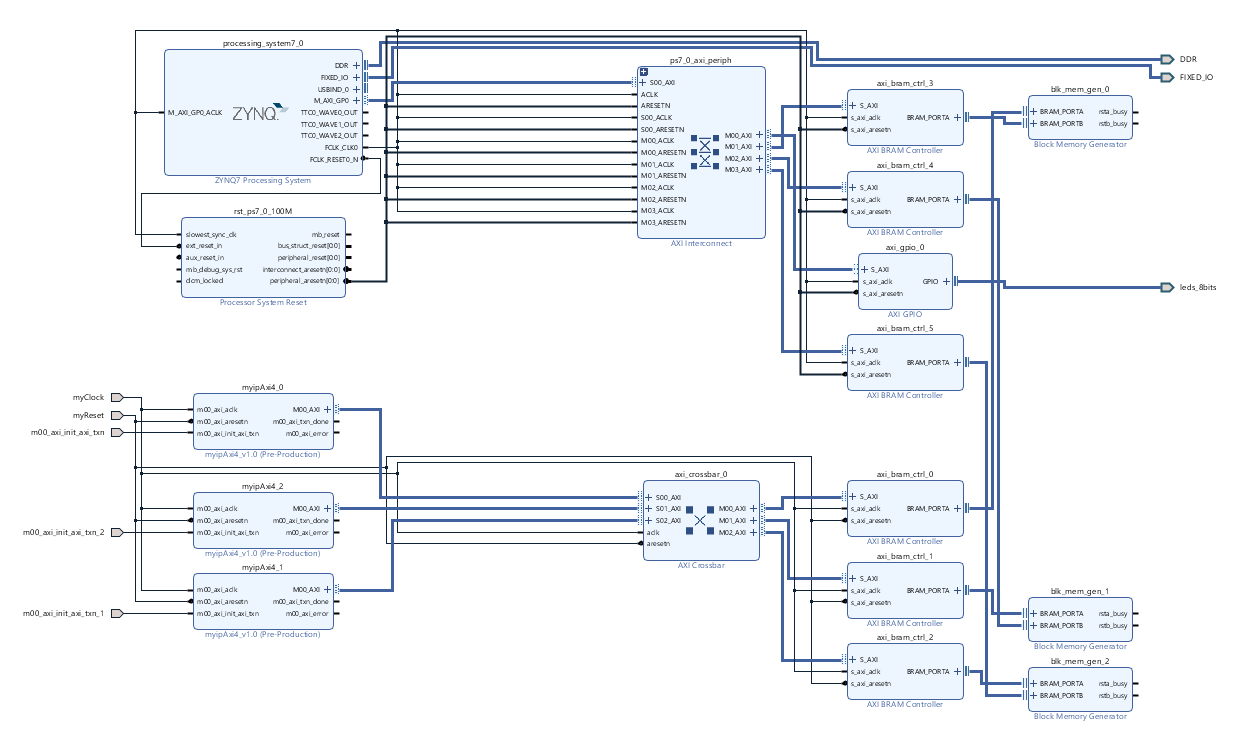
\includegraphics[width=1\textwidth]{./images/NOCZYNQ.png}
    \caption{NOC sur ZYNQ}
\end{figure}
\end{document}
